\section{Summary}

\subsection{C++ Language Essentials Review}
\begin{frame}[fragile]{\emoji{books} C++ Key Features Covered Today}
	\textbf{Object-Oriented Programming Fundamentals}:
	\begin{itemize}
		\item \textbf{Classes \& Objects}: Encapsulation, inheritance, polymorphism
		\item \textbf{RAII Principle}: Resource Acquisition Is Initialization
		\item \textbf{Move Semantics}: Efficient resource transfer with \texttt{std::move}
		\item \textbf{Smart Pointers}: \texttt{unique\_ptr}, \texttt{shared\_ptr} for memory safety
	\end{itemize}

	\vspace{0.5em}
	\textbf{Modern C++ Features}:
	\begin{columns}
		\begin{column}{0.5\textwidth}
			\begin{minted}{cpp}
// Lambda expressions
auto lambda = [](int x) { return x * 2; };

// Auto type deduction
auto result = expensive_function();

// Range-based for loops
for (const auto& item : container) {
    process(item);
}
			\end{minted}
		\end{column}
		\begin{column}{0.5\textwidth}
			\begin{minted}{cpp}
// References vs pointers
int& ref = variable;  // Always valid
int* ptr = &variable; // Can be null

// Template basics
template<typename T>
void process(T&& value) {
    // Perfect forwarding
}
			\end{minted}
		\end{column}
	\end{columns}
\end{frame}

\begin{frame}[fragile]{\emoji{brain} C++ Concurrency Core Concepts}
	\textbf{The Three Pillars of C++ Concurrency}:

	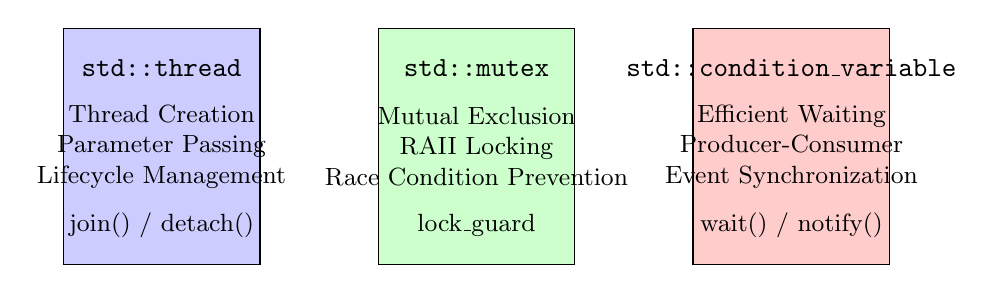
\begin{tikzpicture}
		% Pillar 1: Thread
		\node[draw, rectangle, fill=blue!20, minimum height=3cm, minimum width=2.5cm] (thread) at (0,0) {};
		\node[font=\bfseries] at (0,1) {\texttt{std::thread}};
		\node[font=\small, align=center] at (0,0) {Thread Creation\\Parameter Passing\\Lifecycle Management};
		\node[font=\small] at (0,-1) {join() / detach()};

		% Pillar 2: Mutex
		\node[draw, rectangle, fill=green!20, minimum height=3cm, minimum width=2.5cm] (mutex) at (4,0) {};
		\node[font=\bfseries] at (4,1) {\texttt{std::mutex}};
		\node[font=\small, align=center] at (4,0) {Mutual Exclusion\\RAII Locking\\Race Condition Prevention};
		\node[font=\small] at (4,-1) {lock\_guard};

		% Pillar 3: Condition Variable
		\node[draw, rectangle, fill=red!20, minimum height=3cm, minimum width=2.5cm] (cv) at (8,0) {};
		\node[font=\bfseries] at (8,1) {\texttt{std::condition\_variable}};
		\node[font=\small, align=center] at (8,0) {Efficient Waiting\\Producer-Consumer\\Event Synchronization};
		\node[font=\small] at (8,-1) {wait() / notify()};
	\end{tikzpicture}

	\vspace{1.5em}
	\textbf{Advanced Features}:
	\begin{itemize}
		\item \textbf{C++17 Parallel Algorithms}: \texttt{std::execution::par} for automatic parallelization
		\item \textbf{Thread-Safe Containers}: Building producer-consumer queues
		\item \textbf{Hardware Awareness}: \texttt{thread::hardware\_concurrency()}
	\end{itemize}
\end{frame}

\subsection{C++ Parallel Programming Key Points}
\begin{frame}[fragile]{\emoji{gear} Thread Management Best Practices}
	\textbf{Thread Lifecycle Management}:
	\begin{columns}
		\begin{column}{0.5\textwidth}
			\textbf{Correct Thread Handling}
			\begin{minted}{cpp}
void safe_threading() {
    std::thread t(worker_function);

    // Always ensure join or detach
    if (t.joinable()) {
        t.join();  // Wait for completion
    }

    // Or for fire-and-forget
    // t.detach();
}
			\end{minted}
		\end{column}
		\begin{column}{0.5\textwidth}
			\textbf{RAII Thread Guard}
			\begin{minted}{cpp}
class thread_guard {
    std::thread& t;
public:
    explicit thread_guard(std::thread& t_)
        : t(t_) {}

    ~thread_guard() {
        if (t.joinable()) {
            t.join();
        }
    }
};
			\end{minted}
		\end{column}
	\end{columns}

	\vspace{1em}
	\textbf{Parameter Passing Rules}:
	\begin{itemize}
		\item Arguments are \textbf{copied by default} into thread
		\item Use \texttt{std::ref()} for reference passing
		\item Use \texttt{std::move()} for efficient resource transfer
		\item Be careful with pointer/reference lifetimes
	\end{itemize}
\end{frame}

\begin{frame}[fragile]{\emoji{lock} Synchronization Patterns}
	\textbf{Mutex Usage Patterns}:
	\begin{columns}
		\begin{column}{0.5\textwidth}
			\textbf{Basic Protection}
			\begin{minted}{cpp}
class ThreadSafeCounter {
private:
    int count = 0;
    mutable std::mutex mtx;
public:
    void increment() {
        std::lock_guard<std::mutex> lock(mtx);
        ++count;
    }

    int get() const {
        std::lock_guard<std::mutex> lock(mtx);
        return count;
    }
};
			\end{minted}
		\end{column}
		\begin{column}{0.5\textwidth}
			\textbf{Deadlock Prevention}
			\begin{minted}{cpp}
// Ordered locking
void transfer(BankAccount& from,
              BankAccount& to, double amount) {
    if (&from < &to) {
        std::lock_guard<std::mutex> lock1(from.mtx);
        std::lock_guard<std::mutex> lock2(to.mtx);
    } else {
        std::lock_guard<std::mutex> lock2(to.mtx);
        std::lock_guard<std::mutex> lock1(from.mtx);
    }
    from.balance -= amount;
    to.balance += amount;
}
			\end{minted}
		\end{column}
	\end{columns}

	\vspace{1em}
	\textbf{Producer-Consumer with Condition Variables}:
	\begin{itemize}
		\item Replace busy-waiting with efficient event-driven synchronization
		\item Use \texttt{unique\_lock} for flexible locking with condition variables
		\item Always check conditions in a loop to handle spurious wakeups
	\end{itemize}
\end{frame}

\begin{frame}[fragile]{\emoji{rocket} Modern C++ Parallel Features}
	\textbf{C++17 Parallel Algorithms}:
	\begin{columns}
		\begin{column}{0.6\textwidth}
			\begin{minted}{cpp}
#include <execution>
#include <algorithm>

std::vector<int> data(1000000);
std::iota(data.begin(), data.end(), 1);

// Sequential execution
std::sort(data.begin(), data.end());

// Parallel execution
std::sort(std::execution::par,
          data.begin(), data.end());

// Parallel + vectorized
std::sort(std::execution::par_unseq,
          data.begin(), data.end());
			\end{minted}
		\end{column}
		\begin{column}{0.4\textwidth}
			\textbf{Execution Policies}:
			\begin{itemize}
				\item \texttt{seq}: Sequential
				\item \texttt{par}: Parallel
				\item \texttt{par\_unseq}: Parallel + Vectorized
				\item \texttt{unseq}: Vectorized (C++20)
			\end{itemize}

			\vspace{1em}
			\textbf{Available Algorithms}:
			\begin{itemize}
				\item \texttt{std::for\_each}
				\item \texttt{std::transform}
				\item \texttt{std::reduce}
				\item \texttt{std::sort}
				\item Many others...
			\end{itemize}
		\end{column}
	\end{columns}
\end{frame}
\subsection{Framework Comparison: Morning vs Afternoon}
\begin{frame}[fragile]{\emoji{compass} Parallel Programming Framework Selection}
	\textbf{Decision Tree}:
	\begin{tikzpicture}[node distance=2cm]
		% Main decision point
		\node[draw, diamond, fill=yellow!20] (start) at (0,0) {Parallel Task};

		% First level decisions
		\node[draw, diamond, below left of=start, fill=blue!10] (pattern) {Regular\\Data Pattern?};
		\node[draw, diamond, below right of=start, fill=blue!10] (scale) {Scale\\Requirement?};

		% Solutions
		\node[draw, rectangle, below of=pattern, fill=green!20] (openmp) {\textbf{OpenMP}\\(Morning)};
		\node[draw, rectangle, below left of=scale, fill=red!20] (cpp) {\textbf{C++ Threads}\\(Afternoon)};
		\node[draw, rectangle, below right of=scale, fill=purple!20] (mpi) {\textbf{MPI}\\(Morning)};

		% Arrows with labels
		\draw[->] (start) -- node[above left] {Loop-based} (pattern);
		\draw[->] (start) -- node[above right] {Complex Logic} (scale);
		\draw[->] (pattern) -- node[left] {Yes} (openmp);
		\draw[->] (scale) -- node[above left] {Single Node} (cpp);
		\draw[->] (scale) -- node[above right] {Multi-node} (mpi);
	\end{tikzpicture}
\end{frame}

\begin{frame}{\emoji{vs} Framework Comparison Matrix}
	\begin{table}[h]
		\centering
		\scriptsize
		\begin{tabular}{|l|c|c|c|}
			\hline
			\textbf{Feature}         & \textbf{OpenMP} & \textbf{C++ Threads} & \textbf{MPI} \\
			\hline
			\textbf{Learning Curve}  & \textcolor{green}{Easy}    & \textcolor{orange}{Moderate}     & \textcolor{red}{Hard} \\
			\textbf{Development Time}& \textcolor{green}{Fast}    & \textcolor{orange}{Medium}       & \textcolor{red}{Slow} \\
			\textbf{Control Level}   & \textcolor{red}{Low}       & \textcolor{green}{High}          & \textcolor{green}{High} \\
			\textbf{Memory Model}    & Shared          & Shared               & Distributed \\
			\textbf{Scalability}     & 1-64 cores      & 1-32 cores           & 1000s cores \\
			\textbf{Debugging}       & \textcolor{green}{Easy}    & \textcolor{orange}{Medium}       & \textcolor{red}{Hard} \\
			\hline
			\textbf{Best Use Case}   & Data Parallel   & Producer-Consumer    & HPC Clusters \\
			                         & Loops           & Complex Sync         & Supercomputing \\
			\hline
		\end{tabular}
	\end{table}

	\vspace{1em}
	\textbf{Key Insights}:
	\begin{itemize}
		\item \textbf{OpenMP}: Pragma-based, excellent for parallelizing existing loops
		\item \textbf{C++ Threads}: Fine-grained control, perfect for complex synchronization patterns
		\item \textbf{MPI}: Message passing, designed for distributed memory systems
	\end{itemize}
\end{frame}

\subsection{Practical Implementation Examples}
\begin{frame}[fragile]{\emoji{hammer} Common Parallel Patterns Implementation}
	\textbf{Producer-Consumer Pattern (C++ Threads)}:
	\begin{columns}
		\begin{column}{0.5\textwidth}
			\begin{minted}{cpp}
template<typename T>
class ThreadSafeQueue {
private:
    std::queue<T> queue_;
    mutable std::mutex mutex_;
    std::condition_variable condition_;

public:
    void push(T item) {
        {
            std::lock_guard<std::mutex> lock(mutex_);
            queue_.push(std::move(item));
        }
        condition_.notify_one();
    }

    T pop() {
        std::unique_lock<std::mutex> lock(mutex_);
        condition_.wait(lock, [this] {
            return !queue_.empty();
        });
        T result = std::move(queue_.front());
        queue_.pop();
        return result;
    }
};
			\end{minted}
		\end{column}
		\begin{column}{0.5\textwidth}
			\textbf{Usage Example}:
			\begin{minted}{cpp}
ThreadSafeQueue<int> taskQueue;

// Producer thread
void producer() {
    for (int i = 0; i < 100; ++i) {
        taskQueue.push(i);
        std::this_thread::sleep_for(
            std::chrono::milliseconds(10));
    }
}

// Consumer thread
void consumer(int id) {
    while (true) {
        try {
            int task = taskQueue.pop();
            std::cout << "Consumer " << id
                     << " processing: " << task
                     << std::endl;
            // Process task...
        } catch (...) {
            break;
        }
    }
}
			\end{minted}
		\end{column}
	\end{columns}
\end{frame}

\begin{frame}[fragile]{\emoji{gear} Parallel Reduction Comparison}
	\textbf{Sum Array Elements - Three Approaches}:
	\begin{columns}
		\begin{column}{0.33\textwidth}
			\textbf{OpenMP}
			\begin{minted}{cpp}
long parallel_sum_openmp(
    const std::vector<int>& arr) {
    long sum = 0;

    #pragma omp parallel for \
        reduction(+:sum)
    for (size_t i = 0; i < arr.size(); ++i) {
        sum += arr[i];
    }

    return sum;
}
			\end{minted}
		\end{column}
		\begin{column}{0.33\textwidth}
			\textbf{C++ Threads}
			\begin{minted}{cpp}
long parallel_sum_threads(
    const std::vector<int>& arr) {

    unsigned num_threads =
        std::thread::hardware_concurrency();
    std::vector<std::thread> threads;
    std::vector<long> results(num_threads);

    size_t chunk_size = arr.size() / num_threads;

    for (unsigned i = 0; i < num_threads; ++i) {
        threads.emplace_back([&, i]() {
            size_t start = i * chunk_size;
            size_t end = (i == num_threads - 1) ?
                arr.size() : (i + 1) * chunk_size;

            results[i] = std::accumulate(
                arr.begin() + start,
                arr.begin() + end, 0L);
        });
    }

    for (auto& t : threads) t.join();

    return std::accumulate(
        results.begin(), results.end(), 0L);
}
			\end{minted}
		\end{column}
		\begin{column}{0.33\textwidth}
			\textbf{C++17 Parallel}
			\begin{minted}{cpp}
long parallel_sum_cpp17(
    const std::vector<int>& arr) {

    return std::reduce(
        std::execution::par,
        arr.begin(),
        arr.end(),
        0L
    );
}
			\end{minted}

			\vspace{2em}
			\textbf{Complexity Comparison}:
			\begin{itemize}
				\item OpenMP: 6 lines
				\item C++ Threads: 25 lines
				\item C++17: 4 lines
			\end{itemize}
		\end{column}
	\end{columns}
\end{frame}
\begin{frame}[fragile]{\emoji{dart} Monte Carlo π Calculation: All Frameworks}
	\textbf{Problem}: Estimate π using random point sampling

	\begin{columns}
		\begin{column}{0.3\textwidth}
			\textbf{OpenMP Version}
			\begin{minted}{cpp}
#include <omp.h>
#include <random>

double monte_carlo_openmp(long samples) {
    long count = 0;

    #pragma omp parallel reduction(+:count)
    {
        std::random_device rd;
        std::mt19937 gen(rd());
        std::uniform_real_distribution<> dis(0.0, 1.0);

        #pragma omp for
        for(long i = 0; i < samples; i++) {
            double x = dis(gen);
            double y = dis(gen);
            if(x*x + y*y <= 1.0) {
                count++;
            }
        }
    }

    return 4.0 * count / samples;
}
			\end{minted}
		\end{column}
		\begin{column}{0.35\textwidth}
			\textbf{C++ Thread Version}
			\begin{minted}{cpp}
#include <thread>
#include <vector>
#include <atomic>

std::atomic<long> global_count(0);

void worker(long samples) {
    std::random_device rd;
    std::mt19937 gen(rd());
    std::uniform_real_distribution<> dis(0.0, 1.0);

    long local_count = 0;
    for(long i = 0; i < samples; i++) {
        double x = dis(gen);
        double y = dis(gen);
        if(x*x + y*y <= 1.0) {
            local_count++;
        }
    }

    global_count += local_count;
}

double monte_carlo_cpp(long samples) {
    const int num_threads = std::thread::hardware_concurrency();
    std::vector<std::thread> threads;

    long samples_per_thread = samples / num_threads;

    for(int i = 0; i < num_threads; i++) {
        threads.emplace_back(worker, samples_per_thread);
    }

    for(auto& t : threads) {
        t.join();
    }

    return 4.0 * global_count / samples;
}
			\end{minted}
		\end{column}
		\begin{column}{0.35\textwidth}
			\textbf{MPI Version}
			\begin{minted}{cpp}
#include <mpi.h>

double monte_carlo_mpi(long samples) {
    int rank, size;
    MPI_Comm_rank(MPI_COMM_WORLD, &rank);
    MPI_Comm_size(MPI_COMM_WORLD, &size);

    long local_samples = samples / size;
    long local_count = 0;

    std::random_device rd;
    std::mt19937 gen(rd() + rank);
    std::uniform_real_distribution<> dis(0.0, 1.0);

    for(long i = 0; i < local_samples; i++) {
        double x = dis(gen);
        double y = dis(gen);
        if(x*x + y*y <= 1.0) {
            local_count++;
        }
    }

    long global_count;
    MPI_Reduce(&local_count, &global_count, 1,
               MPI_LONG, MPI_SUM, 0, MPI_COMM_WORLD);

    if(rank == 0) {
        return 4.0 * global_count / samples;
    }
    return 0.0;
}
			\end{minted}
		\end{column}
	\end{columns}
\end{frame}

\begin{frame}[fragile]{\emoji{bar-chart} Performance Analysis}
	\textbf{Benchmark Results} (1 billion samples):

	\begin{table}[h]
		\centering
		\begin{tabular}{|l|c|c|c|c|}
			\hline
			\textbf{Framework} & \textbf{Time (s)} & \textbf{Speedup} & \textbf{Accuracy} & \textbf{LOC} \\
			\hline
			Sequential         & 12.5              & 1.0×             & π ≈ 3.141592      & 15           \\
			OpenMP             & 1.8               & 6.9×             & π ≈ 3.141591      & 20           \\
			C++ Thread         & 1.9               & 6.6×             & π ≈ 3.141593      & 35           \\
			MPI (8 nodes)      & 0.3               & 41.7×            & π ≈ 3.141590      & 40           \\
			\hline
		\end{tabular}
	\end{table}

	\vspace{1em}
	\textbf{Trade-offs Analysis}:
	\begin{itemize}
		\item \textbf{OpenMP}: Best effort/performance ratio for shared memory
		\item \textbf{C++ Thread}: Maximum control, good for complex algorithms
		\item \textbf{MPI}: Unmatched scalability for distributed computing
	\end{itemize}

	\vspace{0.5em}
	\textbf{Development Productivity}:
	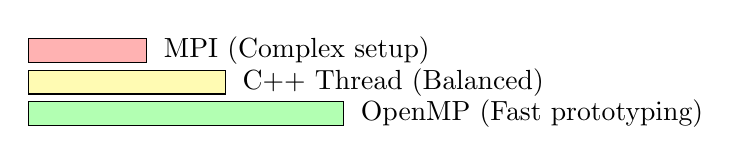
\begin{tikzpicture}
		\draw[fill=green!30] (0,0) rectangle (4,0.3);
		\draw[fill=yellow!30] (0,0.4) rectangle (2.5,0.7);
		\draw[fill=red!30] (0,0.8) rectangle (1.5,1.1);

		\node[right] at (4.1,0.15) {OpenMP (Fast prototyping)};
		\node[right] at (2.6,0.55) {C++ Thread (Balanced)};
		\node[right] at (1.6,0.95) {MPI (Complex setup)};
	\end{tikzpicture}
\end{frame}

\subsection{Advanced Topics Preview}
\begin{frame}[fragile]{\emoji{telescope} Beyond the Basics: Advanced Concurrency}
	\textbf{Topics for Further Exploration}:

	\begin{columns}
		\begin{column}{0.5\textwidth}
			\textbf{Asynchronous Programming}
			\begin{minted}{cpp}
#include <future>

auto future = std::async(std::launch::async,
    []() {
        return expensive_computation();
    });

// Do other work...
auto result = future.get();  // Wait for result
			\end{minted}

			\textbf{Atomic Operations}
			\begin{minted}{cpp}
#include <atomic>

std::atomic<int> counter{0};

void increment() {
    counter.fetch_add(1, std::memory_order_relaxed);
}
			\end{minted}
		\end{column}
		\begin{column}{0.5\textwidth}
			\textbf{Thread Pools}
			\begin{minted}{cpp}
class ThreadPool {
    std::vector<std::thread> workers;
    std::queue<std::function<void()>> tasks;
    std::mutex queue_mutex;
    std::condition_variable condition;

public:
    template<class F>
    void enqueue(F&& f) {
        {
            std::lock_guard<std::mutex> lock(queue_mutex);
            tasks.emplace(std::forward<F>(f));
        }
        condition.notify_one();
    }
};
			\end{minted}
		\end{column}
	\end{columns}

	\vspace{1em}
	\textbf{Learning Path}:
	\begin{enumerate}
		\item Master the basics: \texttt{thread}, \texttt{mutex}, \texttt{condition\_variable}
		\item Explore \texttt{std::async} and \texttt{std::future}
		\item Study atomic operations and memory models
		\item Implement lock-free data structures
		\item Build thread pools and work-stealing algorithms
	\end{enumerate}
\end{frame}

\subsection{Key Takeaways}
\begin{frame}[fragile]{\emoji{star} Today's Essential Learning Points}
	\textbf{C++ Concurrency Trinity}:
	\begin{enumerate}
		\item \textbf{\texttt{std::thread}}: Thread creation and lifecycle management
		\item \textbf{\texttt{std::mutex}}: Race condition prevention with RAII
		\item \textbf{\texttt{std::condition\_variable}}: Efficient event-driven synchronization
	\end{enumerate}

	\vspace{1em}
	\textbf{Programming Paradigm Shift}:
	\begin{columns}
		\begin{column}{0.5\textwidth}
			\textbf{From Sequential Thinking}:
			\begin{itemize}
				\item Single execution path
				\item Direct variable access
				\item Simple debugging
				\item Predictable timing
			\end{itemize}
		\end{column}
		\begin{column}{0.5\textwidth}
			\textbf{To Concurrent Thinking}:
			\begin{itemize}
				\item Multiple execution paths
				\item Synchronized data access
				\item Complex interactions
				\item Non-deterministic timing
			\end{itemize}
		\end{column}
	\end{columns}

	\vspace{1em}
	\textbf{Framework Selection Summary}:
	\begin{itemize}
		\item \textbf{Quick prototyping}: Use OpenMP for data-parallel loops
		\item \textbf{Fine control}: Use C++ threads for complex synchronization
		\item \textbf{Massive scale}: Use MPI for distributed computing
		\item \textbf{Modern C++}: Use parallel algorithms for standard operations
	\end{itemize}
\end{frame}

\begin{frame}[fragile]{\emoji{motorway} Next Steps in Your Parallel Programming Journey}
	\textbf{Immediate Practice}:
	\begin{itemize}
		\item Implement the producer-consumer pattern from today's examples
		\item Convert a sequential algorithm to use parallel STL algorithms
		\item Experiment with the parallel execution assignment (NVIDIA HPC SDK)
	\end{itemize}

	\vspace{1em}
	\textbf{Advanced Topics to Explore}:
	\begin{columns}
		\begin{column}{0.5\textwidth}
			\begin{itemize}
				\item \textbf{Memory Models}: Understanding memory ordering
				\item \textbf{Lock-free Programming}: Using atomics effectively
				\item \textbf{Thread Pools}: Efficient task management
				\item \textbf{Async/Future}: Modern asynchronous patterns
			\end{itemize}
		\end{column}
		\begin{column}{0.5\textwidth}
			\begin{itemize}
				\item \textbf{GPU Programming}: CUDA, OpenCL, SYCL
				\item \textbf{Distributed Computing}: Advanced MPI patterns
				\item \textbf{High-Level Frameworks}: Intel TBB, OpenCV parallel
				\item \textbf{Performance Analysis}: Profiling and optimization
			\end{itemize}
		\end{column}
	\end{columns}

	\vspace{1em}
	\textbf{Remember}: Start simple, measure performance, and gradually add complexity!
\end{frame}
